\subsection{Extension Cr\'eateur de grille}

% when the revision of a section has been finalized, 
% comment out the following line:
% \updatedisclaimer

% The graticule creator allows to create a ``grid'' of points or polygons to
% cover our area of interest. All units must be entered in decimal degrees.
% The output is a shapefile which can be projected on the fly to match your
% other data.
Le cr\'eateur de grille permet de cr\'eer une ``grille'' de points ou de polygones
pour couvrir notre zone d'int\'er\^et. Toutes les unit\'es doivent \^etre entr\'ees en
degr\'es d\'ecimaux. Le format de sortie est le shapefile qui peut \^etre projet\'e \`a la
vol\'ee pour correspondre \`a vos donn\'ees.

\begin{figure}[ht]
\begin{center}
%   \caption{Create a graticule layer
  \caption{Cr\'eer une couche de grille
\nixcaption}\label{fig:graticule}\smallskip
  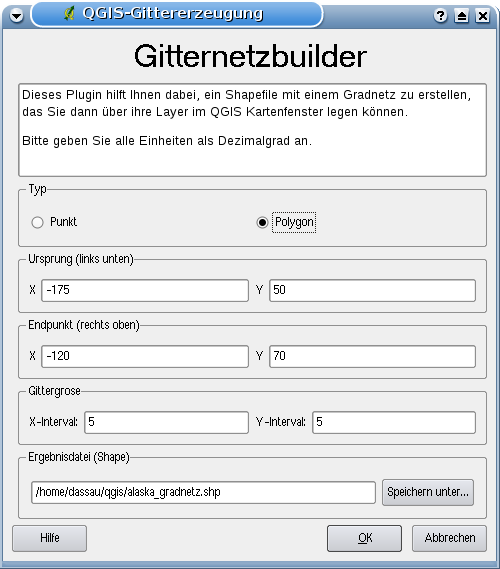
\includegraphics[clip=true, width=10cm]{grid_maker_dialog}
\end{center}
\end{figure}

% Here is an example how to create a graticule:
Voici un exemple pour cr\'eer une grille :

\begin{enumerate}
% \item Start QGIS, load the Graticule Creator Plugin in the Plugin Manager (see
% Section \ref{sec:load_core_plugin}) and click on the
% \toolbtntwo{grid_maker}{Graticule Creator} icon which appears in the QGIS
% toolbar menu.
\item D\'emarrez QGIS, charger l'extension "Cr\'eation de grille" dans le
Gestionnaire de plugin (voir la section~\ref{sec:load_core_plugin}) et cliquez
sur l'ic\^one \toolbtntwo{grid_maker}{Cr\'eateur de grille}  qui apparait dans la
barre de menu QGIS.
% \item Choose the type of graticule you wish to create: point or polygon.
\item Choisissez le type de grille que vous voulez cr\'eer : point ou polygone.
% \item Enter the latitude and longitude for the lower left and upper right
% corners of the graticule.
\item Entrez la latitude et la longitude pour les coins bas-gauche et
haut-droit de la grille.
% \item Enter the interval to be used in constructing the grid. You can enter
% different values for the X and Y directions (longitude, latitude)
\item Entrez l'intervalle \`a utilis\'e dans la construction de la grille. Vous
pouvez entrer diff\'erentes valeurs pour les directions X et Y (longitude,
latitude).
% \item Choose the name and location of the shapefile to be created.
\item Choisissez le nom et le r\'epertoire du shapefile \`a cr\'e\'e.
% \item Click \button{OK} to create the graticule and add it to the map canvas.
\item cliquez sur \button{OK} pour cr\'eer la grille et l'ajouter \`a la carte.
\end{enumerate} 



